\begin{enumerate}
  \item Definiční obor (může být zadán na intervalu)
  \item Derivace
  \item Nulové body derivace $f'(x)=0$
    \begin{enumerate}[label=(\alph*)]
      \item vypočítat
      \item vyjde konkrétní výsledek
      \item musí být v interavalu D(f)
    \end{enumerate}
  \item K nul. bodům D(f) přidáme hodnotu z $f'(x)=0$
  \item Do funkce f(x) zadáváme hodnoty x z nul. bodů
\end{enumerate}
\subsubsection{Globální extrémy - příklady}
\begin{equation}
  f(x)=\sqrt{2+x}+\sqrt{6-x}
\end{equation}
\hrule
\begin{align*}
  f'(x)&=\frac{\sqrt{6-x}-\sqrt{2+x}}{2*\sqrt{2+x}*\sqrt{6-x}}=0\\
  &=\sqrt{6-x}-\sqrt{2+x}=0\\
  x&=2\in\langle-2;6\rangle
\end{align*}
\begin{center}
  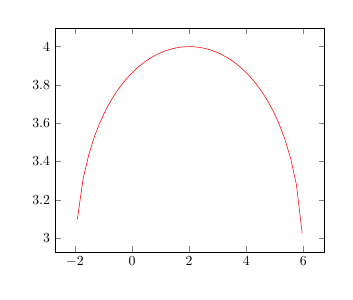
\begin{tikzpicture}[scale=0.5]
    \begin{axis}
      \addplot[color=red,domain=-10:10,samples=100]{sqrt(2+x)+sqrt(6-x)};
    \end{axis}
  \end{tikzpicture}
\end{center}

a) dosadím nulové body do funkce
\begin{center}
  \begin{tikzpicture}[scale=0.5]
    \draw (-2,0) -- (6,0);
    \foreach \x in {-2,2,6} {
      \draw (\x,0.5) -- (\x,-0.5) node[below] {\x};
    }
  \end{tikzpicture}
\end{center}

\begin{tabular}{ c l r } 
$\nearrow$ & $f(-2)=\sqrt{2-2}+\sqrt{6-(-2)}=\sqrt{8}$ & neostré absolutní minimum \\
$\searrow$ & $f(2)=\sqrt{2+2}+\sqrt{6-2)}=4$ & ostré absolutní minimum \\
$\nearrow$ & $f(6)=\sqrt{2+6}+\sqrt{6-6)}=\sqrt{8}$ & neostré absolutní minimum \\
\end{tabular}

\begin{tabular}{c c}
\end{tabular}

b) v případě, že mi vychází nevyčíslitelná hodnota

\begin{center}
  \begin{tikzpicture}[scale=0.5]
    \draw (-2,0) -- (6,0);
    \foreach \x in {-2,2,6} {
      \draw (\x,0.5) -- (\x,-0.5) node[below] {\x};
    }
    \foreach \x/\s/\t in {0/+/\nearrow,4/-/\searrow} {
      \draw (\x,0.5) node{\s};
      \draw (\x,-0.5) node{$\t$};
    }
  \end{tikzpicture}
\end{center}
